\chapter{Physics: Scaling Cell-Based Assays} % Write in your own chapter title
\label{Chap:Physics}
\begin{figure}[!b]
\centering
\begin{tabular}{c}
$t = 0.0\,$s 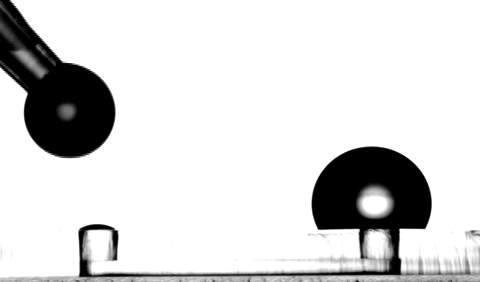
\includegraphics[width=2in]{PP_1.png} \cr
$t = 0.4\,$s 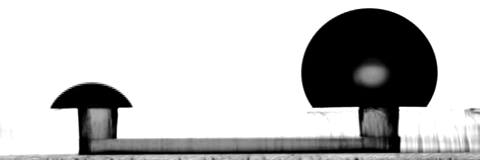
\includegraphics[width=2in]{PP_2.png} \cr
$t = 4.0\,$s 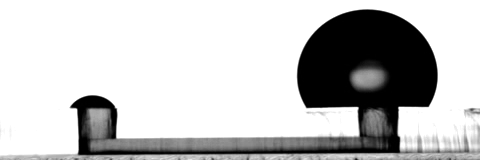
\includegraphics[width=2in]{PP_3.png} \cr
\end{tabular}
\caption{\textbf{Passive-pumping}. Images represent a time series originally taken by movie by Keil Regehr observing passive pumping using a Goniometer, an instrument for measuring the profiles of interfaces. Some frames of the movie are included here to illustrate fluid pumping in a microchannel using a manual pipette. In accordance with the Young-Laplace equation for the internal pressure of a droplet, the small droplet pumps towards the large droplet. The majority of the pumping occurs in less than a second while the remainder occurs as the wetted perimeter of the input droplet settles to a final diameter. Typically, the port radius or the protein adsorbed region surrounding the port defines the wetted perimeter, essentially eliminating the last phase equilibration of the wetted perimeter as compared to these images.}
\label{chap1:fig:passivePumping}
\end{figure}
This chapter summarizes efforts to characterize some basic advantages and challenges for micro-scale approaches to cell culture. Challenges include microchannel washing and evaporation while potential advantages include reduced volumes and control of diffusive transport. However, a brief mention of passive-pumping is necessary to put the following studies into context and is a terrific example of how a reduction in scale can affect the balance of physical forces, leading to new approaches for cell-based assays. 

As the volumes of fluids used for cell-based assays are reduced, the influence of gravity on the shape and flow of those fluids is reduced relative to surface tension. The Young-Laplace equation defines the pressure within a droplet with a curvature of radius, $R$, in a system with a surface tension constant of $\gamma$ (Eq \ref{chap1:equ:youngLaplace}). Passive-pumping has been thoroughly characterized by previous lab members \cite{Berthier:2007mi,Walker:2002ez}; however, an extensive appendix of equations used to model droplet geometries, pressures, volumes, and heights is provided to avoid others having to repeat this effort (Appendix \ref{App:DropletGeometry}).

\begin{equation}
\Delta P = \frac{\gamma}{2 R}
\label{chap1:equ:youngLaplace}
\end{equation}

%%%%%%%%%%%%%%%%%%%%%%
%%%%%%%%%%%%%%%%%%%%%%
%%%%%        Laminar Flow     %%%%%%%
%%%%%%%%%%%%%%%%%%%%%%

\section{Laminar Flow: Channel Washing and Treatments}
\paragraph{Preface.}The information in this section is adapted or summarized from \cite{Warrick:2007lq}.\\
\\
\noindent One of the first questions that is typically asked by a new user of microchannels is, ``How much fluid should I use to wash out the microchannel?'' The question is an important one for cell-based assays and is challenging given the parabolic flow profile characteristic of low Reynolds number flow (Fig \ref{chap1:fig:washing}A). At the boundary of the channels, the velocity of the fluid is zero, thus resulting in fluid left behind during washing. Fluorescent beads and food coloring were used to characterize the ability to remove this boundary layer via passive-pumping. Experimental results agree with an analytical model of laminar flow that predicts \% washing of the channel, $\Phi$, given the volume of the channel, $V_{channel}$, and the volume of the fluid used to wash the channel, $V_{wash}$ (Eq \ref{chap1:equ:washing}) \cite{Warrick:2007lq}. 
\begin{equation}
\Phi = 1 - \zeta\frac{V_{channel}}{V_{wash}}
\label{chap1:equ:washing}
\end{equation}
Numerical simulation is used to obtain the value of $\zeta$ which is a constant that depends upon the cross-sectional geometry of the channel. The value of $\zeta$ for different cross-sections is plotted in Fig \ref{chap1:fig:washing}B for reference. Additional considerations are treated in the manuscript on this subject such as the use of a wash-wait-wash methodology to leverage diffusion to increase washing efficiency.

\begin{figure}[!ht]
\centering
\begin{tabular}{p{0.3cm}cp{0.3cm}c}
A)&\imagetop{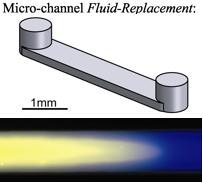
\includegraphics[height=1.5in]{Wells_and_Microchannels_2_Cropped.png}}&B)&\imagetop{\includegraphics[height=1.5in]{Zeta.pdf}}
\end{tabular}
\caption{\textbf{Fluid replacement in a microchannel}. A) Schematic of simple one-input-one-output microchannel and the characteristic parabolic shape of low Reynolds number fluid flow in microchannels. B) Washing constant, $\zeta$, plotted for various aspect ratios for microchannels with rectangular cross-section, $h/w$.}
\label{chap1:fig:washing}
\end{figure}

%%%%%%%%%%%%%%%%%%%%%%
%%%%%%%%%%%%%%%%%%%%%%
%%%%%        Evaporation       %%%%%%%
%%%%%%%%%%%%%%%%%%%%%%

\section{Evaporation: Theory and Implications}
\paragraph{Preface.}The information presented in this section is adapted or summarized from \cite{Berthier:2008jf,Berthier:2008tl}.\\
\\
\noindent Given the exposed fluid in passive-pumping-based devices, another question commonly fielded is, ``How do I keep evaporation from affecting my cells?'' Even in an incubator, a significant percentage of the microchannel volume can evaporate without additional measures. In previous work, we highlight that evaporation is surprisingly proportional to the radius of an exposed droplet instead of the surface area, as can be seen in Eq \ref{chap1:equ:evaporation} where $D$ is the diffusion coefficient of water vapor in air, $\Delta C_{sat}$ is the difference between the saturation concentration of water in air and the atmospheric concentration, and $R$ is the droplet radius.

\begin{equation}
E = \frac{2 \pi D}{\rho} \Delta C_{sat} R = \lambda R 
\label{chap1:equ:evaporation}
\end{equation}

In a passive-pumping-based channel, fluid typically flows from the smaller droplet to the larger droplet as seen in the top of Fig \ref{chap1:fig:evaporationSchematic}. However, as a evaporation begins to affect the volume of fluid in each drop, the surface tension attempts to keep the curvature at each port the same. This results in fluid flow back towards the input drop (Fig \ref{chap1:fig:evaporationSchematic}, bottom). This was first documented as a way to concentrate protein by Walker \etal\ and has since been used by Frisk \etal\ to increase the sensitivity of detection of botulinum neurotoxin \cite{Walker:2002oy,Frisk:2008pi}.

\begin{figure}[!ht]
\centering
\includegraphics[width=3.5in]{EvaporationSchematic.pdf}
\caption{\textbf{Evaporation-driven flow}. Schematic illustration of typical surface-tension driven flow using a pipette (top) and evaporation-driven flow (bottom).}
\label{chap1:fig:evaporationSchematic}
\end{figure}


From Eq \ref{chap1:equ:evaporation}, a dimensionless evaporation number, $Ev$, can be developed that represents the proportion of fluid that is lost over the time-course of an experiment for an array of droplets (see manuscripts for details) \cite{Berthier:2008jf,Berthier:2008tl}. Experiments validated this model which was then used to help characterize different ways to mitigate evaporation. As one might expect, in an array of droplets, the droplets at the perimeter incur the largest percent change in volume. Thus, for a given proportion of fluid lost from an array as predicted by the $Ev$ number, say 10\%, the majority of that 10\% is lost from the perimeter droplets. In this scenario, one can define a penetration depth of the evaporation effects. This penetration depth was numerically simulated and is shown in Fig \ref{chap1:fig:evaporation2} for different aspect ratio containers. From this information, it can be seen that the use of sacrificial fluid near the perimeter in low profile containers is an effective way to mitigate evaporation for passive-pumping-based devices. Further, the nesting of containers also adds another layer of protection against evaporation.

\begin{figure}[!ht]
\centering
\includegraphics[width=3.5in]{Evaporation_Exptl2.pdf}
\caption{\textbf{Evaporation from micro-device arrays}. Evaporation in containers of various aspect ratio used to house arrays of micro-devices with exposed fluid or droplets. For a given amount of fluid lost from the entire array (denoted by $Ev$), penetration depth is given for different \% losses. The penetration depth for 1\% of $Ev$ is roughly half the container radius for a container with an aspect ratio ($H/R$) of 0.1. Thus, all droplets outside a distance of $R/2$ are expected to see a loss of greater than 1\% of $Ev$.}
\label{chap1:fig:evaporation2}
\end{figure}

%%%%%%%%%%%%%%%%%%%%%%
%%%%%%%%%%%%%%%%%%%%%%
%%%%%        Reduced Volumes   %%%%%
%%%%%%%%%%%%%%%%%%%%%%

\section{Reduced Volumes: The Promise of Microfluidics}

\paragraph{Preface.}The information presented in this section is adapted or summarized from \cite{Warrick:2008rf}.\\
\\
\noindent One of the primary benefits of microfluidics is the reduced volumes needed to perform an assay, which can lead to reductions in assay footprints, cost, and the number of cells needed to perform an assay. This allows one to begin exploring larger parameter spaces with a given cell sample and is an important advantage in the areas of primary cell work and clinical diagnostics and will be important in addressing more complex biological hypotheses that require multi-parametric or combinatorial experimental designs. In this respect, Fig \ref{chap1:fig:scales} helps to put passive-pumping or tube-less microfluidics in perspective with other microfluidic approaches. Passive-pumping-based devices do not use the smallest volumes or have the highest potential for throughput but offer an important advantage similar to multi-well plates; they can be operated manually or integrated with existing pipette automation. This ability is very important for facilitating translation of new assays from the bench-top to the high-throughput screening facility. 

\begin{figure}[!ht]
\centering
\includegraphics[width=3.5in]{MicrofluidicsScales.pdf}
\caption{\textbf{Microfluidic platforms for screening}. Plot of approximate volumes-per-chamber across a range of spatial densities using different types of devices. The figure shows ranges of operation for traditional multi-well plates, tubeless microchannels, tubed/valved microchannels, and droplet-based devices (see Section X for descriptions and references). Tube-less microchannels can offer a reduction in volume-per-assay compared to multi-well formats of similar density but can still preserve the ability to individually address an assay compared to tubed/valved devices that use the same volume. Volume-per-assay increases for tubed/valved microchannels when implemented to individually address chambers due to increases in dead volumes, routing, tubing, or numbers of connected reservoirs, whereas multiplexing of fluid sources decreases the average volume-per-assay. Droplet-based fluidics typically deals with volumes below a few \textmu L and has the potential to manipulate picoliter volumes at high densities.}
\label{chap1:fig:scales}
\end{figure}

Besides increasing the number of experiments you can do with a given sample, the use of reduced volumes also affects the cellular microenvironment. As volumes reduce, the effective culture volume or ECV generally decreases (Fig \ref{chap1:fig:cellVolumeRatio}); that is to say, the volume of culture media per cell decreases. This decreased ECV gives the cell more control over its microenvironment. The cells can more quickly condition their microenvironment, resulting in more rapid accumulation and depletion of factors, nutrients, and waste. This effect has been used to increase the sensitivity of co-culture assays to uncover cell signaling effects that could not be seen before \invitro\ \cite{Domenech:2009jt}.

\begin{figure}[!ht]
\centering
\includegraphics[width=3.5in]{CellVolumeRatio.pdf}
\caption{\textbf{Effective culture volume (ECV) or volume-per-cell in 2-D and 3-D culture}. A) Schematic representation of cells uniformly seeded in 3-D culture and the associated ECV. $L$ is roughly the average spacing between cells. B) Example of different 2-D culture devices and their associate ECVs. The microchannel, tissue-culture flask, co-culture transwell, and 96-well plate in the photo are put in order of increasing ECV. If, in each case, the cells are plated at the same surface density upon the culture substrate (i.e., cells/mm ), then ECV is proportional to the fluid height over the cells.}
\label{chap1:fig:cellVolumeRatio}
\end{figure}

Lastly, by avoiding the use of tubes, passive-pumping-based microfluidics reduces `dead-volumes' and enables arrays of individually addressable devices. Individually addressable devices prevent any potential issues of `cross-talk' that can occur if the devices are connected in any way using tubing and valves. Another benefit is that interaction between devices is completely flexible and configurable via pipetting allowing fluid to be transferred at any time between any two channels.

%%%%%%%%%%%%%%%%%%%%%%
%%%%%%%%%%%%%%%%%%%%%%
%%%%%        Diffusion     %%%%%%%%%
%%%%%%%%%%%%%%%%%%%%%%
\section{Diffusion: Soluble Factor Signaling and Co-culture}

\paragraph{Preface.}This work was written in partnership with Erwin Berthier and represents a manuscript in preparation.\\
\\
\noindent Much in the same way that surface tension effects are more important on the micro-scale, so is diffusion. Across small distances diffusion can happen very quickly. In the case of synapses, factors diffuse to induce signaling in a matter of milliseconds. Given this difference, micro-scale technology has provided a variety of advanced techniques for tailoring the \emph{in vitro} microenvironment of cells to answer unique and specific questions that can be difficult or impossible to answer using macroscale analogs \cite{Chen:1998xq,Lucchetta:2005kn}. The area of segregated co-culture is particularly exciting given the increased sensitivity and flexibility of micro co-culture assays for examining soluble factor signaling between two or more cell types. Segregated co-culture in microdevices typically realize these improvements over standard macroscale technology (\emph{i.e.} transwells) through reduced signaling distances, the ability to precisely pattern cells, independent control of cell number \emph{v.s.} cell density, and increases in the number of cells per unit of culture volume \cite{Bhatia:1999ta,Domenech:2009jt,Folch:2000tb,Nelson:2002ev}. However, up to this point, more focus has been placed on providing unique capabilities instead of ways to objectively compare these new alternatives. Specifically, the literature is lacking a widely applicable tool for assessing the suitability of a particular device for a given co-culture scenario or for the reverse, providing insight into co-culture signaling dynamics based on culture results in a particular device design.

Analyses of soluble factor signaling in the literature are often aimed at very specific or detailed scenarios that are difficult to apply to other situations, even if closely related, while others can be too simplistic and cannot provide an adequate representation or are not tailored enough to the application of co-culture. The analysis provided here can be generalized to a wide range of relevant situations and considers the important but measurable characteristics of cellular sensitivity and soluble factor degradation. This method is a practical tool for both assessing the ability of co-culture device to support signaling between two cell populations as well as assessing the soluble factor production and sensitivity of cell types cultured using a particular device. In this way, the work presented here is significantly relevant and practical for both biologists and engineers and can also apply to other co-culture-like assays such as those for wound-healing or migration.

Fig \ref{chap1:fig:cocultureSchematic}A shows the major steps and processes involved in a paracrine interaction. Factors diffuse between cells through a gap ranging from nm's to mm's to initiate signaling. In the simplest case, a unique factor is produced\slash secreted\slash accumulated on one side and is received\slash sensed\slash taken up by the other (Fig \ref{chap1:fig:cocultureSchematic}A). 
\begin{figure}[!b]
\centering
\begin{tabular}{p{0.3cm}cp{0.3cm}c}
A)&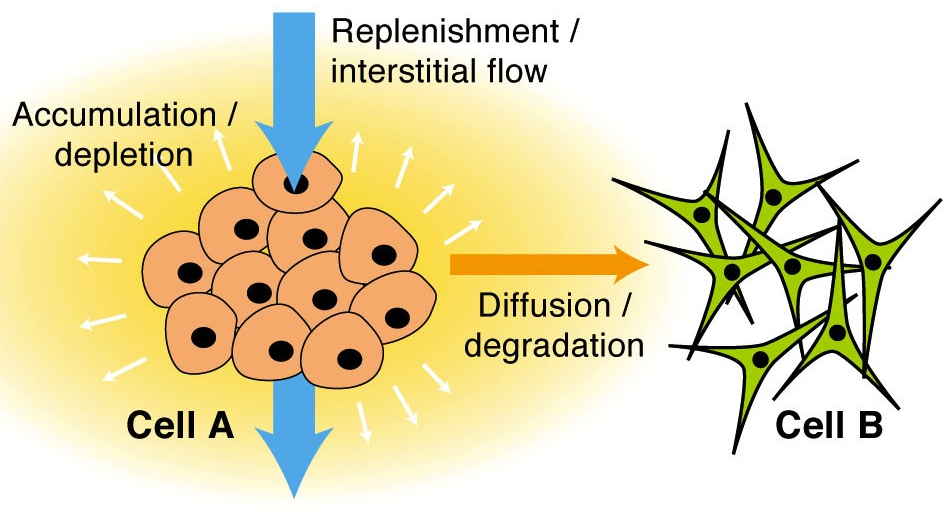
\includegraphics[width=2.5in]{DiffusionIntro_Cropped.jpg}&B)&\includegraphics[width=2.5in]{MathModel.pdf}
\end{tabular}
\caption{\textbf{Co-culture diffusion}. A. Schematic of the simplified coculture model used for analysis. The curvature in the concentration profile of the one dimensional model is evidence of degradation.}
\label{chap1:fig:cocultureSchematic}
\end{figure}
The processes of accumulation, transport, and depletion are dynamic, each with their own rate and associated timescale. There are also timescales and sensitivities associated with cell signaling and response. Design of co-culture assays must account for each of these timescales and sensitivities to enable robust observation of co-culture interactions between populations. Conversely, an understanding of these co-culture parameters can be used to give insight into the nature of an observed interaction in a particular device. Fig \ref{chap1:fig:cocultureSchematic}B is generalized schematic of how the soluble factor interactions of Fig \ref{chap1:fig:cocultureSchematic}A are modeled\slash studied \emph{in vitro} and forms the basis for a practical and widely applicable analysis of co-culture. Soluble factor \emph{transport} in the gap between the populations and the \emph{local culture environment} of the cells in each chamber will be modeled independently and linked in a discussion of timescales of co-culture signaling. A model of transport is developed first given the necessity of transport in paracrine interactions.

\subsection{Transport}
\subsubsection{Math Model}
\label{SubSubSection:MathModel}
The mathematical basis of the proposed transport model is described and used to compare the performance of multiple microscale co-culture devices. In the model shown in Fig \ref{chap1:fig:cocultureSchematic}B, there is a population of cells secreting a soluble factor that can be sensed by a population of receiving cells. In order to make the model both practical and applicable to a wide variety of situations, assumptions are made to simplify calculations and make it easier to estimate system parameters. First, it is assumed that the factor must reach a threshold concentration, $C_{thresh}$, in the receiving chamber in order for signaling to occur. Second, at steady-state, the secreting cells are able to maintain a local concentration of $C_{source}$. As the factors diffuse from one side to the other they also degrade (see curved lines in Fig \ref{chap1:fig:cocultureSchematic}B plot). We can model the process of diffusion and take into account degradation using Eq \ref{equ:diffusion} where $C$ is the concentration [mol/m$^{3}$], $k$ is the degradation constant [1/s], $D$ is the diffusion coefficient [m$^{2}$/s], and $x$ is the distance from the secreting cells [m]. We can use this model to evaluate device designs and determine for a particular factor whether signaling will be efficient or even possible. The 1-D model is most applicable for scenarios where the height and depth of the gap region is less than or equal to the height and depth of the culture chambers (Fig \ref{chap1:fig:cocultureSchematic}A).


%\begin{figure}[!t]
%\centering
%\includegraphics[width=3.2in]{cocultureAnalysis.jpg}
%\caption{Analytical results using a simplified model of segregated coculture. A. The ratio of the actual exchange rate of soluble factors to the maximum possible exchange rate for various geometries and diffusion coefficients is plotted. The ratio is calculated for a ratio of $C_{thresh}/C_{source}=0.1$. B. Plot of $L_/L_{\tau}$ when $\dot{N}_{L}/\dot{N}_{max} = 0$ (\emph{i.e.}, when soluble factor exchange is 0 but the concentration over the sensing cells is able to reach $C_{thresh}$. Thus, this represents the maximum possible distance over which signaling can occur for a particular coculture scenario, $L_{max}/L_{\tau}$. The dotted line represents $L_{max}/L_{\tau}$ when $C_{thresh}/C_{source}=0.1$ -- the same scenario as plotted in part A.}
%\label{chap1:fig:coculture}
%\end{figure}

\begin{equation}
\frac{\partial C}{\partial t} = D\,\frac{\partial^{2} C}{\partial x^{2}} - k C
\label{equ:diffusion}
\end{equation}

We are interested finding $\dot{N}_{L}$, the flux of molecules into the receiving culture chamber (i.e. the number of moles being delivered per unit time at $x=L$, where $L$ is the distance between the two cultures). $\dot{N}_{L}$ is given by Eq \ref{equ:ficks} in terms of the characteristic parameters of the co-culture system. The dimensionless coefficient $\alpha$ varies between 0 and 1 and represents how much degradation of the diffusing molecules attenuates flux. $D$ describes the influence of the medium through which a particular molecule diffuses (e.g. a molecule diffuses more quickly through typical cell culture media than a collagen matrix). The quantity $A/L$ represents the influence of geometry (i.e. more flux occurs through a short channel with a large cross-section versus a long and narrow channel) whereas $\Delta C$ encompasses the influence of the cells on the system.

\begin{equation}
\dot{N}_{L} = \alpha \, D \left(\frac{A}{L} \right) \Delta C
\label{equ:ficks}
\end{equation}

\begin{equation}
\Delta C = C_{source}-C_{thresh}
\label{equ:deltaC}
\end{equation}

\begin{equation}
\alpha=\frac{\mathcal{L}}{1-\mathcal{C}}\left(\frac{1-\mathcal{C}\cosh(\mathcal{L})}{\sinh(\mathcal{L})}\right)
\label{equ:alpha}
\end{equation}

\begin{equation}
\mathcal{C} = \frac{C_{thresh}}{C_{source}}
\label{equ:C}
\end{equation}

\begin{equation}
\mathcal{L} = \frac{\sqrt{k}L}{\sqrt{D}} = 1.18\frac{L}{L_{\tau}} = \frac{\sqrt{ln(2)}}{\sqrt{\tau}}\frac{\,L}{\sqrt{D}}\frac{\sqrt{2}}{\sqrt{2}} = 1.18\frac{L}{\sqrt{2 D \tau}} = 1.18\frac{L}{L_{\tau}}
\label{equ:L}
\end{equation}

\begin{equation}
L_{\tau}= \sqrt{2 D \tau}
\label{equ:lTau}
\end{equation}

When the solution to $\dot{N}_{L}$ is put into this form, it can be seen that the influence of degradation on co-culture signaling (i.e. the value of $\alpha$) depends upon two important dimensionless parameters, $L/L_{\tau}$ and $C_{thresh}/C_{source}$ (Eq \ref{equ:alpha}-\ref{equ:lTau}). The distance $L_{\tau}$ represents the average distance a molecule will diffuse in one half-life (Eq \ref{equ:lTau}). The half-life of the molecule, $\tau$, is given by ln(2)/$k$ where $k$ is the degradation rate in Eq \ref{equ:diffusion}. When $L/L_{\tau} \approx 0$, degradation is negligible, and when $L/L_{\tau} > 1$, degradation of the soluble factor significantly diminishes the rate of delivery to the receiving cells. The ratio of $C_{thresh}/C_{source}$ for a given $L_{\tau}$ determines the maximum possible distance at which signaling can be maintained, $L_{max}$ (Eq \ref{equ:lMax}). Beyond a distance of $L_{max}$, concentration of the factor falls below $C_{thresh}$ due to degradation, cutting off signaling. Lastly, the time it takes for a signal to travel a distance $L$ is approximately $L^{2}/(10\,$D) while the time it takes to reach equilibrium over that distance is roughly $L^{2}/(2\,$D).

\begin{equation}
L_{max} = 0.85 \, L_{\tau} \, \textrm{arccosh}\left(\frac{1}{\mathcal{C}}\right)
\label{equ:lMax}
\end{equation}

The only non-linear term in the calculation of $\dot{N}_{L}$ is $\alpha$, which is plotted in Fig \ref{chap1:fig:alpha} for a range of $L/L_{\tau}$ and $C_{thresh}/C_{source}$. This information is will be used to compare different co-culture device designs.

\begin{figure}[!t]
\centering
\includegraphics[width=3.2in]{Alpha.pdf}
\caption{\textbf{Degradation coefficient, $\alpha$}. Plot of $\alpha$, for different values of $L/L_{\tau}$ and $C_{thresh}/C_{source}$. Black triangles indicate the maximum signaling distance that can be maintained for each value of $C_{thresh}/C_{source}$ (i.e. $L_{max} = 2.5 L_{\tau}$ for $C_{thresh}/C_{source}$ = 0.1).}
\label{chap1:fig:alpha}
\end{figure}

\subsubsection{Comparison of Device Designs}

\def\imagetop#1{\raisebox{1em}{\vtop{\null\hbox{#1}}}}
\begin{table*}[!t]
\caption{\textbf{Comparison of soluble factor delivery in various microscale co-culture designs}. Comparisons are made for a generic short half-life soluble factor ($\tau=30$ [min], D = 100 [$\mu$m$^{2}$/s] in media). The last column, $\dot{N}_{L}/d$, is the rate of molecular transport into the receiving culture chamber \emph{per unit length} $d$. The length $d$ is measured along the length of the interface between the two cultures. The delivery rates can be used to estimate the efficacy of each design relative to one another. Calculations assume $C_{thresh}/C_{source}=0.1$.}%$L_{max}$ for this scenario is 880 $\mu$m.
\centering
\begin{tabular}{p{2cm}@{\,}p{2.7cm}@{\,}p{3.2cm}@{\,}>{\centering}p{1.2cm}@{\,}>{\centering}p{1.2cm}@{\,}>{\centering}p{1.5cm}@{\,}>{\centering}p{1cm}@{\,}>{\centering}p{2cm}}\toprule Method & Embodiment & Schematic & Height\newline$h$\newline[$\mu$m] &  Length\newline$\;\;L$\newline[$\mu$m] & Diff. Coeff.\newline D\newline[$\mu$m$^{2}$/s] & Deg. Coeff.\newline$\alpha$ & Delivery Rate\newline$\;\;\dot{N}_{L}/d$\newline[pmol/(m\,s)] \cr \midrule
Laminar flow patterning & \imagetop{\includegraphics[height= 1.4cm]{LaminarMethod.pdf}} &\imagetop{\includegraphics[height=1.4cm]{LaminarSchematic.pdf}} & 250 & 250 & 100 & 0.95 & 95$\,\Delta C$ \cr 
Segregated co-culture & \imagetop{\includegraphics[height= 1.4cm]{SegregatedMethod.pdf}} &\imagetop{\includegraphics[height= 1.4cm]{SegregatedSchematic.pdf}} & 12.5 & 500 & 100 & 0.81 & 2.0$\,\Delta C$ \cr 
Gel-separated co-culture & \imagetop{\includegraphics[height= 1.4cm]{GelMethod.pdf}} &\imagetop{\includegraphics[height= 1.4cm]{GelSchematic}} & 250 & 750 & 20 & 0 & 0$\,\Delta C$ \cr 
\bottomrule
\end{tabular}
\label{tab:examples}
\end{table*}

Using this model, we can practically and objectively compare different device designs for a particular co-culture scenario (Tab \ref{tab:examples}). In order to compare the transport of soluble factor in each device, a value is calculated for $\dot{N}_{L}$. However, the length of the interface between the cell populations ($d$) is different for each device. For this reason, we present the rate of transport per unit length of the device (i.e. $\dot{N}_{L}/d$). The devices are compared assuming the factor of interest is a relatively short-lived protein with a diffusivity typical of many growth factors ($\tau$ = 30 [min], D = 100 [$\mu$m$^{2}$/s]). It is also assumed that the secreting cells produce a relative abundance of the factor compared to the sensitivity of the receiving cells (i.e. $C_{thresh}/C_{source}$ = 0.1).

% Table Calcs for alpha
%(sqrt(2*100e-12*30*60))
%    r151 = 0.0006
%1.18/r151
%    r152 = 1966.66666667
%((250e-6*r152)/(1-0.1))*((1-0.1*cosh((250e-6*r152)))/(sinh((250e-6*r152))))
%    r154 = 0.947653018885
%((500e-6*r152)/(1-0.1))*((1-0.1*cosh((500e-6*r152)))/(sinh((500e-6*r152))))
%    r153 = 0.805564568799
%(sqrt(2*20e-12*30*60))
%    r148 = 0.0002683281573
%1.18/r148
%    r149 = 4397.60035575
%((750e-6*r149)/(1-0.1))*((1-0.1*cosh((750e-6*r149)))/(sinh((750e-6*r149))))
%    r150 = -0.0962824670932

%Table Calcs for Ndot/d = alpha D h / L
% 0.947653018885*100*250/250
% 0.805564568799*100*12.5/500
% 0*20*250/750

The highest transport per unit length (95$\Delta C$) was calculated for the case of laminar flow patterning where the cell populations were in close proximity and with little or no constriction or barrier to diffusion between them. Degradation of the short half-life molecule was negligible ($\alpha \approx 1$). By constricting the region between cells and doubling the distance between the cells, transport was cut by factor of 1/50 (see segregated co-culture). Degradation was not the major factor in the segregated case; instead, the constriction used to separate the populations severely limited transport. In the case of the gel-separated co-culture, $\alpha$ was $\le 0$, suggesting that signaling is impossible in this scenario. Diffusion of the factor in gel is significantly slower than in media such that, over a distance of 750 $\mu$m, the secreting cells could not produce a concentration $\ge C_{thresh}$ in the receiving cell culture chamber due to degradation.

Although some devices prove more effective than others in this example, other situations might prove the designs to be relatively interchangeable, such as with small, long lived molecules like hormones. There is also the question of timing. Can the molecule accumulate to appropriate concentrations and diffuse to the receiving population in a short enough time to observe cell response upon acquiring a specific readout? Will uptake or media replenishment significantly attenuate signaling? To begin answering these questions, the local environment of each cell population is examined.

%$\dot{N}_{L}$ depends on the cross sectional area of the gap region, $A$; diffusion coefficient, D; characteristic length ratio, $L/L_{\tau}$; and ratio of the receiving chamber concentration to the source chamber concentration, $C_{thresh}/C_{source}$. $C_{thresh}$ is used for the concentration in the receiving culture chamber because the goal of the co-culture device is to adequately supply the receiving cells with enough factor to illicit a response and very often a threshold concentration can be associated with this response. When $\alpha$ approaches 1, degradation is insignificant and exchange is maximal. When the value approaches 0, either the constriction\slash barrier between the culture chambers or degradation of soluble factors over the distance $L$ is preventing significant transport. When the value actually reaches 0, a value of $C_{thresh}$ can no longer be sustained in the receiving culture chamber, making signaling impossible. 

%$\dot{N}_{L}/\dot{N}_{max}$ can be used to compare devices in two ways. The first way compares performance relative to a common $\dot{N}_{max}$ (the higher of the two $\dot{N}_{max}$'s calculated for each device) and the other uses values of $\dot{N}_{max}$ that are specific to each device. The first method is a direct comparison of specific geometries while the second allows one to compare devices if they were to be scaled such that the culture chamber heights were the same. In this way, the second is more appropriate for comparing methods rather than specific device designs, such as the use of constrictions \emph{vs} gel barriers to segregate populations. In order to compare two devices with different geometries, one can calculate $\dot{N}_{L}/\dot{N}_{max}$ If two different devices have the same value of $\dot{N}_{L}/\dot{N}_{max}$, then they can equally support soluble factor signaling for a given co-culture scenario if the culture chamber heights were made to be similar.

%A simple graphical method is provided to perform these comparisons using only the heights of the culture chamber and gap region as well as the diffusion coefficient and half-life of the molecule of interest.

%Within the plot of $\dot{N}_{L}/\dot{N}_{max}$ in Fig \ref{chap1:fig:cocultureSchematic}A, colored and numbered dots are plotted that represent the efficiency of soluble factor exchange for each device shown in Fig \ref{chap1:fig:cocultureSchematic}B for two different factors -- one with a short half-life and one with a long half-life. Given the disparity of the points, one can begin to seen that soluble factor exchange can be dramatically different depending on the molecule and coculture geometry. The plot shows that the LFP device presented here (device 1) produces nearly maximal exchange of factors and avoids issues of factor degradation. On the contrary, \mbox{IL-2} signaling is impossible in device 3 as $L/L_{\tau}$ is greater than $L_{max}/L_{\tau}$. 

\subsection{Local Culture Environment}

Although transport between the cell populations is critical for observing soluble factor interactions, it is also important to understand the dynamics of the local environments of each population in culture as they determine the boundary conditions of the transport model from the previous section (i.e. $C_{thresh}$ and $C_{source}$). We can use well-studied models of soluble factor secretion and uptake to give a sense of these dynamics for designing co-culture assays. Models of platelet-derived growth factor (PDGF) accumulation and epidermal growth factor (EGF) depletion will be used for this purpose and are discussed along with the influence of cell density. The models approximate the local environment of a cell in 2-D culture (i.e. culture on a flat substrate instead of in a 3-D matrix) as being a cylinder where the radius of the cylinder depends upon the cell density and the height of the culture chamber (Fig \ref{chap1:fig:diffusionGeom}, see Appendix \ref{App:Diffusion} for description of simulation methods).

The PDGF and EGF models in this section require 3-D diffusion modeling (COMSOL modeling sofware, Burlington, MA) and the knowledge of factor production/uptake rates, which can be difficult to measure. Therefore, the intent is not to describe to the reader how to do this type of modeling; instead, the examples will be used to discuss the timescales of accumulation and depletion and how different parameters affect those processes. In this way, some practical guidelines can be suggested from specific examples. Also, these models examine the dynamics of a single culture chamber and do not account for transport between two culture chambers. The interaction between culture chambers depends on the conditions in each chamber as $C_{source}$ and $C_{thresh}$ determine the boundary conditions of the co-culture signaling model. Further, the time-scale of accumulation and depletion within each chamber determine when co-culture signaling is likely to occur.

\begin{figure}[!t]
\centering
\includegraphics[width=3.5in]{CylindricalChannel.pdf}
\caption{\textbf{Cylindrical diffusion model geometry}. The cylindrical geometry in the schematic used to estimate the case of a single cell in culture with neighbors on a 2-D substrate. The geometry is modeled in COMSOL using a 2-D axis symmetrical model with a flux boundary condition at the cell surface defined as $q$. The area of the base of the unit-cylinder is equal to the area-per-cell on the substrate of the channel. Parameters of the model were determined from the literature and noted in figure captions.}
\label{chap1:fig:diffusionGeom}
\end{figure} 

\subsubsection{PDGF Accumulation}

Fig \ref{chap1:fig:PDGF} shows modeling results for fibroblastic cells (10$\mu$m in diameter) producing platelet-derived growth factor (PDGF) at a rate, $q$, reported in simulations and experimental work from the literature (cite Lauffenburger - cell density and Leof). Concentration is plotted with time for the cell boundary, $C_{cb}$; the ceiling of the channel (i.e. approximately the point of lowest concentration); and the average concentration over the entire channel. The simulation assumes that cells are seeded at 300 cells/mm$^{2}$ ($\sim 30\%$ confluency or $\sim 65$ $\mu$m spacing). The channel height, $H$, is chosen to be 250 $\mu$m ($\gg$ the $5\mu$m cell radius). Although the dissociation constant of PDGF to its receptor does not always predict the concentrations necessary for cellular response, it is used here to estimate a cellular threshold concentration, $C_{th}$. Initially, the concentration near the cell builds quickly showing local accumulation of the factor. However, soon the difference between the average channel concentration and the cell boundary concentration stabilizes at $t_{d}=H^{2}/(2\,D)$. Each measure of concentration then rises at a rate of $q/V$ where $V$ is the volume of the modeled cylinder. 


\begin{figure}[!b]
\centering
\includegraphics[width=3.5in]{PDGF.pdf}
\caption{\textbf{Production of PDGF by fibroblasts.} Plot of concentration with time for the parameters listed in the plot. Parameters are taken from \cite{Lauffenburger:1989fy,LEOF:1986uq} (see Appendix \ref{App:Diffusion} for more details).}
\label{chap1:fig:PDGF}
\end{figure}

The average concentration in the channel reaches $C_{thresh}$ in $\le 30$ min, at which point the concentration at the cell boundary is $\sim 35\%$ higher. However, this percent difference quickly becomes negligible as PDGF continues to rapidly accumulate. The calculations here assume there is no depletion due to adsorption, absorption, uptake, degradation, or cellular feedback mechanisms that might reduce production. Despite these assumptions, it becomes apparent that the cells in this microscale culture model can quickly affect their local environment due to a high cell to culture-volume ratio (i.e. the culture chamber height is small). If the height of the fluid over the cells were to be like that in a typical culture flask (2 mm), accumulation would occur 8 times slower (2 mm / 0.25 mm = 8). Thus, instead of reaching $C_{thresh}$ in just 30 min, it would take approximately 4 hours in a culture flask.

\subsubsection{EGF Depletion}

\begin{figure}[!b]
\centering
\includegraphics[width=3.5in]{EGF.pdf}
\caption{\textbf{Uptake of EGF by fibroblasts.} Plot of concentration with time for the parameters listed in the plot. The geometry of the simulation is shown in Fig \ref{chap1:fig:diffusionGeom}. Parameters are taken from \cite{KNAUER:1984fj,STARBUCK:1992kl} (see Appendix \ref{App:Diffusion} for more details).}
\label{chap1:fig:EGF}
\end{figure}

Fig \ref{chap1:fig:EGF} shows the reverse case of EGF uptake of by human fibroblasts (HFs). The same parameters exist for the EGF example as for the PDGF example, but with different values. The production rate is negative here to signify uptake rather than release. Also, although the dissociation constant of EGF to its receptor is often quoted as $10^{-10}$ to $10^{-9}$, it has been observed that the apparent cellular affinity for EGF is $\sim 4.69 \times 10^{-11}$, possibly due to cellular regulation of surface receptors (cite Lauffenburger). The initial concentration of EGF in the culture medium is chosen to be $4 \times C_{th}$ for illustrative purposes. The plot shows that cells uptake the EGF linearly until concentrations approach $C_{th}$ whereupon the sigmoidal response of the cell is observed to reduce uptake due to depletion of the medium. Thus, it can be seen that cellular uptake rates for small values of $V$ can cause rapid depletion of threshold levels of factor. The medium becomes significantly depleted $< 1$ [hr] after reaching $C_{th}$. This time is relatively short compared to the 6-8hrs of exposure often required to illicit a growth response. Therefore, when $V$ is too small, depletion can make it impossible to examine dose response to steady concentrations of soluble factors. However, if the initial concentration, $C_{0}$, is high enough initially, saturating exposure can be achieved for significant periods of time until the threshold concentration is reached whereupon depletion quickly occurs.

\subsubsection{Single Chamber Accumulation/Depletion and Local Cell Density}
\label{SubSubSection:LocalGradients}

As mentioned in the previous examples, local concentration is significantly affected by seeding density or cell spacing. Since the total volume of the channel is constant, the rate of accumulation increase linearly with the number of cells seeded into a chamber. This also means that normal random dispersion on the culture substrate can significantly affect local accumulation and depletion. Locally (i.e. within the neighborhood of a group of cells), accumulation\slash depletion rates can vary by many multiples due to cell slumping that arises from the stochastic nature of cell suspensions and seeding or by the natural growth and reorganization of cells during culture. However, the influence of these local variations is quickly diminished given that the average concentration in the channel can quickly surpass threshold concentrations or can be quickly depleted, thereby homogenizing cell-response throughout the chamber.

\subsection{Co-culture Timescales}

Four important timescales to consider for the study of co-culture interactions are the time for accumulation in the secreting chamber, the time for diffusion across the gap, the half-life of the molecule, and the timescale of the phenotypic change to be measured in the receiving chamber. The times are listed in this order as they mirror the typical sequence of events from secretion, to transport and degradation, to uptake and response. If any of these timescales does not agree with the readout or limits the process of soluble factor signaling, it is possible that the device geometry might be changed to minimize this constraint and enable more robust signaling. Further, geometric changes might be used to modulate a signaling event to gain additional insight.

Methods are available to estimate these times, especially when testing the effects of a specific factor. Accumulation times per volume of fluid can typically be estimated using an ELISA or other similar readout. A diffusion coefficient is necessary and can typically be estimated using the molecular weight of the molecule if no information is available in the literature (see Einstein–Stokes equation). However, a typical 20kD protein is usually in the range of 100 \textmu m$^{2}$/s in fluid similar to media or water. A time for diffusion can then be estimated as $t_{d} = L^{2}/(2D)$ where $L$ is the distance of interest such as the gap width. Half-life information can often be found in the literature as well but can also be measured for secreted factors using an ELISA. If diffusion times across the gap are on the order of degradation times, it is worth performing the analysis outlined and described in Section \ref{SubSubSection:MathModel}. The $C_{source}$ needed for the analysis in that section can come from the ELISA accumulation data whereas the $C_{thresh}$ is more easily determined from dose-response curves obtained in mono-culture using an exogenous source of the protein. The dose-response data also will likely provide the time-scale of the phenotypic response being measured. The co-culture assay should be performed over a long enough time to allow accumulation, transport, and response.

If the factor is unknown, different designs can be used to alter these timescales and gain in general information about the unknown factor. For example, if signaling is achieved, one can assume that the degradation coefficient, $\alpha$, of Section \ref{SubSubSection:MathModel} is $>$ 0. The value of $\alpha$ can then be estimated for potential candidate molecules to narrow the scope of further inhibition studies to identify the factor. If one can observe a difference in response using narrow and wide gaps, one can support hypotheses of the size or degradation rate of the putative factor. By using different culture chamber sizes to vary the ratio of secreting and receiving cells, insight into secretion rates and sensitivity of the receiving cells can be gained. However, basic considerations of waste production and nutrient depletion can also change when exploring these various permutations. Also, in contrast to the discussion in Section \ref{SubSubSection:LocalGradients}, factor concentrations and response within the receiving chamber can be inhomogeneous and lead to further insight, as explained below.

The results shown in Tab \ref{tab:examples} illustrate that delivery of a co-culture factor to the receiving cell chamber can sometimes be quite limited. In the receiving chamber, the gap acts like a localized source of factor where the factor must diffuse throughout the receiving chamber to influence the population. Depending on the distance of a cell from the gap, the cell could experience a concentration of factor significantly different than its neighbors closer or farther from the gap. This local gradient is different than the local gradient of the previous subsection on accumulation and depletion. In this case, the limited flux through the gap can result in a gradient of factor within the dose-response range of the receiving cells that can last for significant periods of time or potentially reach a quasi-steady-state. For this reason, a dose response may be observed within the receiving chamber. If cells are in close proximity to the gap, diffusion times will be reduced, limiting the potential for these gradients. If the flux through the gap is relatively large, accumulation in the receiving chamber will occur more quickly and help to homogenize response as well.

\subsection{Other Microenvironmental Considerations}
Microscale devices are often made of materials that are different from macroscale tools. Different materials and the reduced scale of the culture devices can lead to changes in the microenvironment that are important to be aware of. A common material for micro-devices is polydimethylsiloxane, which has been shown to have a high capacity for absorbing small lipophilic molecules such as estrogen, an important soluble factor in many disease models \cite{Regehr:2009fk}. Also, the surface to volume ratio of micro-devices is significantly increased. Thus, adsorption alone can significantly deplete low concentrations of soluble factors \cite{Lionello:2005zh}.

\subsection{Conclusions}
Microscale techniques offer new ways to probe soluble factor signaling interactions and dynamics with increased sensitivity yet we lack accessible, informative, and widely applicable methods to assess these interactions. These types of analysis methods are needed to aid design and interpretation of co-culture devices and assays to further leverage the potential advantages of microscale co-culture. A model and discussion of co-culture transport was provided here to address this need. The model includes source and threshold concentrations of factor as well as degradation, an often overlooked but important part of soluble factor signaling regulation. By including these components into the model, the analysis gains accuracy and flexibility while avoiding the complexity of more involved methods of analysis. The influence of degradation is summarized in a single dimensionless value that can be estimated from the equations and plot provided. Each parameter of the system can be estimated from the literature or via standard ELISA experiments. Devices were compared using the model and illustrate the importance of micro-device geometry in promoting robust co-culture signaling. The importance of four different timescales (accumulation\slash depletion, transport, degradation, and cell response) were discussed, highlighting how each can be used in aiding design of co-culture devices as well as how they can be used to interpret co-culture results and observations.  

%\section{Extras}
%\clearpage
%
%%%%%%%%%%%%%%%%%%%%%%%%
%
%\paragraph*{Cell:Volume Ratio and Diffusion Distances.}Cell:volume ratio refers to the number of cells being cultured to the volume of media in which they are being cultured. The cell:volume ratio in microscale devices is typically 4 - 10 times higher in microscale culture devices than more standard devices such as culture flasks or micro-well plates. Increased cell:volume ratios allow soluble factors to build up more rapidly. This means that dilution of signaling molecules is prevented and biologically relevant concentrations of these factors are reached more quickly.
%
%The diffusion distance between two cell populations in co-culture is an important consideration given the short half-lives of many siganling molecules (\emph{e.g.}, IL-2, 7 min; slkdfjlskdf). Given the half life of a particular molecule ($\tau$), the distance the molecule can diffuse during a single half life ($L_{\tau}$) can be estimated using $L_{tau} = \sqrt{2 D \tau}$, where $D$ is the diffusion coefficient. Given that typical diffusion coefficients for soluble factors are on the order of 100 \textmu m$^{2}$/s and half lives range from 0.1-2 hours, typical values for $L_{\tau}$ are $\sim$250 - 1200 \textmu m. 
%
%\paragraph*{Maximizing Exchange of Soluble Factors.}The extent of soluble factor exchange between the patterned cell populations can be modulated by adjusting the distance between them or by changing the height of the region in the space between populations. These parameters are illustrated in a cross-section view of a basic microchannel co-culture device (Fig \ref{chap1:fig:coculture}). The co-culture system can be roughly approximated as having one concentration in the region near the producing cells and a second concentration near the receiving cells with a difference of $\Delta C$. Employing Fick's Law of diffusion, Eq \ref{equ:ficks} can be used to relate the molecular transport rate ($\dot{N}$, [mol/s]) between the populations to the concentration gradient ($\partial C/\partial x$) and the cross-sectional area (A) through which the molecules must diffuse to reach the other side. 
%
%\begin{equation}
%\frac{\partial C}{\partial t} = D\,\frac{\partial^{2} C}{\partial x^{2}} - k C
%\end{equation}
%
%\begin{equation}
%\dot{N} = D\,\frac{\partial C}{\partial x} A
%\end{equation}
%
%\begin{equation}
%\dot{N}_{max} = D\,\frac{\Delta C}{L} A
%\end{equation}
%
%\begin{equation}
%\textrm{half-life} = \tau = \frac{\ln(2)}{k}
%\end{equation}
%
%\begin{equation}
%\mathcal{L} = \frac{\sqrt{k}L}{\sqrt{D}} = \frac{\sqrt{ln(2)}}{\sqrt{\tau}}\frac{\,L}{\sqrt{D}}\frac{\sqrt{2}}{\sqrt{2}} = 1.18\frac{L}{\sqrt{2 D \tau}} = 1.18\frac{L}{L_{\tau}}
%\end{equation}
%
%\begin{equation}
%\mathcal{L}_{max} = \textrm{arccosh}\left(\frac{1}{\mathcal{C}}\right) %= -\ln\left({\frac{C_{1}}{C_{2}}-\sqrt{\left(\frac{C_{1}}{C_{2}}\right)^{2}-1}}\right) = \textrm{arccosh}\left(\frac{C_{1}}{C_{2}}\right) 
%\end{equation}
%
%\begin{equation}
%L_{\tau}= \sqrt{2 D \tau}
%\end{equation}
%
%\begin{equation}
%\mathcal{\dot{N}_{\mathrm{L}}}=\frac{\dot{N}_{L}}{\dot{N}_{max}}= \frac   {\left(D \frac{\partial C}{\partial x}A\right)\big|_{x=L}}   {\left(D \frac{\Delta C}{L} A\right)}
%\end{equation}
%
%\begin{equation}
%\mathcal{A}=\frac{A}{A_{max}}
%\end{equation}
%
%\begin{equation}
%\mathcal{C}=\frac{C_{2}}{C_{1}}
%\end{equation}
%
%\begin{equation}
%\mathcal{\dot{N}_{\mathrm{L}}}=\frac{\mathcal{A}\mathcal{L}}{1-\mathcal{C}}\left(\frac{1-\mathcal{C}\cosh(\mathcal{L})}{\sinh(\mathcal{L})}\right) = \mathcal{A}\alpha
%\end{equation}
%
%%\begin{equation}
%%\frac{\dot{N_{2}}}{\dot{N_{2,max}}}=\frac{h}{h_{max}}\frac{\frac{L}{L_{\tau}}}{1-\frac{C_{1}}{C_{2}}}\left(\frac{1-\frac{C_{1}}{C_{2}}\cosh(\frac{L}{L_{\tau}})}{\sinh(\frac{L}{L_{\tau}})}\right)
%%\end{equation}
%%\begin{equation}
%%\frac{\dot{N_{2}}}{d}=D\frac{\alpha h}{L}\left(\frac{C_{1}-C_{2}\cosh(\alpha)}{\sinh(\alpha)}\right)
%%\end{equation}
%%\begin{equation}
%%C_{a}+C_{b} = C_{1}
%%\end{equation}
%%\begin{equation}
%%C_{b} = \frac{C_{1}e^{\frac{L} {\sqrt{\tau D}}}-C2}   {e^{\frac{L} {\sqrt{\tau D}}}-e^{\frac{-L} {\sqrt{\tau D}}}}
%%\end{equation}
%%\begin{equation}
%%C_{a} = C_{1} - \frac{C_{1}e^{\frac{L} {\sqrt{\tau D}}}-C2}   {e^{\frac{L} {\sqrt{\tau D}}}-e^{\frac{-L} {\sqrt{\tau D}}}}
%%\end{equation}
%
%%h = 1;
%%C = 0.01;
%%L = linspace(0,5,50);
%%Ratio = (h).*(L).*(1/(1-C)).*((1-(C).*cosh(L))./(sinh(L)));
%%plot(L,Ratio);
%%drawnow;
%
%
%k is the degradation rate (i.e. 0.1 of C is degraded per unit time)
%
%
%For a given $\Delta C$, as the distance between the cells decreases (\emph{i.e}, $\Delta x \downarrow$) the amount of soluble factor that gets delivered per unit time to the other side increases. By keeping the height of the microchannel between the groups of cells equal with the height of the culture regions, transport of signaling factors between the populations is maximized. Similarly, the use of gel barriers or filters increase the resistance to transport by either changing the effective value of $D$ or $A$. Using the patterning method of Fig \ref{chap1:fig:experimental2}, the space between the cells and resistance to diffusive transport are much reduced compared to transwell assays and help to establish effective soluble factor communication in co-cultures.
%
%\subsection*{Important Identities}
%
%\begin{equation}
%2\cosh (\beta) = e^{\beta}+e^{-\beta}
%\end{equation}
%
%\begin{equation}
%2\sinh (\beta) = e^{\beta}-e^{-\beta}
%\end{equation}
%
%\begin{equation}
%\mathrm{arccosh} (\beta) = \ln\left(\beta + \sqrt{\beta^{2} - 1}\right)
%\end{equation}
%
%%can also be adjusted to modulate the amount of soluble factor exchange as well as . This can be seen using Fick's Law of diffusion which can be used to calculate the moles of soluble factor delivered per unit time ($\dot{N}$) at steady-state from one group of cells to another .
